% !TeX spellcheck = en_US
\addscenariosection{1}{Alliance Scenario}{Brothers in Arms}{\images/chain_of_lightning.png}

\begin{multicols*}{2}

\textbf{Author:} Kolartastic

\textbf{Source:} \href{https://discord.com/channels/740870068178649108/1161571991732625468/threads/1164804609605390386}{Archon Studios Discord}

\textit{Stand together. Fight together. Die together.}  % no-check-caps

\subsection*{\MakeUppercase{Scenario Length}}
12 Rounds

\subsection*{\MakeUppercase{Player Setup}}
\textbf{Player Count:} 4 (2vs2 Alliance)

\textbf{Starting Resources:} 20 \svg{gold}, 3 \svg{building_materials}, 1 \svg{valuables}

\textbf{Starting Income:} 10 \svg{gold}, 0 \svg{building_materials}, 0 \svg{valuables}

\textbf{Starting Units:}

\begin{itemize}
  \item A Few of the cheapest \bronze\ Units
  \item A Few of the cheapest \silver\ Units
\end{itemize}

\textbf{Town Buildings:} \bronze\ Dwelling

\textbf{Additional Starting bonus:}
Choose one:
\begin{itemize}
  \item Search (3) the Ability Deck
  \item A Few \bronze\ Units of the second highest Recruitment cost
\end{itemize}

\textbf{Map Tile Pool:} Each player takes one random Far (II–III) Map Tile.

\subsection*{\MakeUppercase{Map Setup}}
Take the following Map Tiles and arrange them as shown in the Scenario map layout:

\begin{itemize}
  \item 4 × Starting (I) Map Tiles
  \item 2 × Far (II–III) Map Tiles
  \item 4 × Near (IV–V) Map Tiles
  \item 3 × Center (VI–VII) Map Tiles (one with a Dragon Utopia, one with a Grail)
\end{itemize}

\subsection*{\MakeUppercase{Victory Conditions}}
Capture both enemy Starting Towns -- the game ends immediately.
If no team manages to do so, at the end of the \nth{12} Round, select one player from each team to engage in final Combat.

\subsection*{\MakeUppercase{Timed Events}}
\textbf{\nth{4} Round:}
\begin{itemize}
  \item Remove all Black Cubes from the Map.
\end{itemize}
\textbf{\nth{6} and \nth{9} Rounds:}
\begin{itemize}
  \item All players may trade resources or artifacts with one other player.
\end{itemize}

\subsection*{\MakeUppercase{Additional Rules}}
\begin{itemize}
  \item If two allied Heroes are on adjacent Fields, they can freely trade resources, Units and Artifacts.
  \item \textbf{Dragon Utopia:} Gain one Neutral Dragon you defeated.
  \item While posessing the \textbf{Grail Token}, your \svg{hand} limit is increased to 10.
\end{itemize}

\vspace*{\fill}
\hspace*{-1.5em}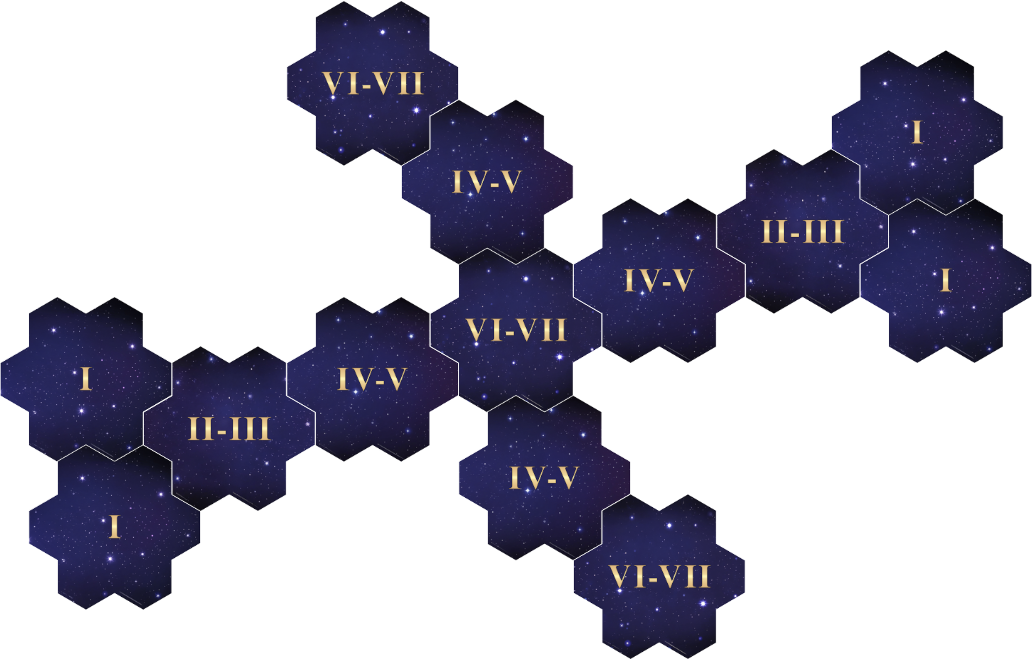
\includegraphics[width=1.1\linewidth]{\maps/brothers_in_arms.png}
\end{multicols*}
